\documentclass[convert = false, tikz]{standalone}
\usepackage[utf8]{inputenc}
\usepackage{tikz}
\usetikzlibrary{automata, positioning, arrows}
 
\usepackage{../../../../style_automata}

% arara: pdflatex
% arara: latexmk: { clean: partial }
\begin{document}
    \tikzset{
    node distance=2.5cm, % specifies the minimum distance between two nodes.
    }
    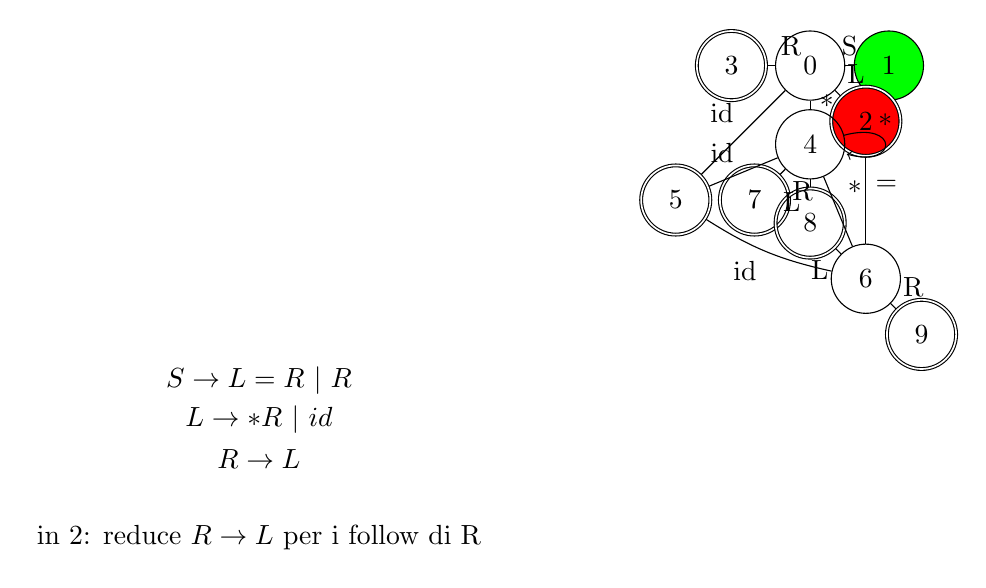
\begin{tikzpicture}
        \node[state] (0) {0};
        \node[align=right] at (-7, -4) {$S \to L=R\ |\ R$};
        \node[align=right] at (-7, -4.5) {$L \to *R\ |\ id$};
        \node[align=right] at (-7, -5) {$R \to L$};
        \node[align=right] at (-7, -6) {in 2: reduce $R \to L $ per i follow di R};
        \node[state, fill=green, right of=0] (1) {1};
        \node[state, fill=red, accepting, below right of=0] (2) {2};
        \node[state, accepting, left of=0] (3) {3};
        \node[state, below of=0] (4) {4};
        \node[state, accepting, below left of=4] (7) {7};
        \node[state, accepting, left of=7] (5) {5};
        \node[state, accepting, below of=4] (8) {8};
        \node[state, below right of=8] (6) {6};
        \node[state, accepting, below right of=6] (9) {9};
        \draw (0) edge[above] node{S} (1)
        (0) edge[above right] node{L} (2)
        (0) edge[above right] node{R} (3)
        (0) edge[right] node{*} (4)
        (0) edge[above left] node{id} (5)
        (2) edge[above right] node{=} (6)
        (4) edge[loop right, above] node{*} (4)
        (4) edge[above left] node{id} (5)
        (4) edge[below right] node{R} (7)
        (4) edge[below left] node{L} (8)
        (6) edge[above right] node{*} (4)
        (6) edge[below left, bend left=10] node{id} (5)
        (6) edge[below left] node{L} (8)
        (6) edge[above right] node{R} (9)
        ;

    \end{tikzpicture}
\end{document}

